% ============================================================
%  华中科技大学实验报告 LaTeX 模版
%  编译：xelatex main.tex（连续两次以更新目录与引用）
%  风格：纯黑白，表格横向铺满版心
% ============================================================

\documentclass[a4paper,12pt]{article}

% ============================================================
%  实验报告 LaTeX 模版 — 导言区配置
%  编译：xelatex main.tex（连续两次以更新目录与引用）
%  风格：纯黑白印刷，用字号/粗细/间距区分层次，不用颜色
% ============================================================

% ============================================================
%  补充宏包与自定义命令
%  注意：页面、表格、代码、颜色等核心配置见 preamble.tex
% ============================================================

% --- 数学公式 ---
\usepackage{amsmath}

% --- 浮动体强制放置 [H] ---
\usepackage{float}

% --- 边距调整（\begin{addmargin}...\end{addmargin}）---
\usepackage{scrextend}

% --- 多栏排版 ---
\usepackage{multicol}

% --- 按名称引用（\nameref）---
\usepackage{nameref}

% --- 附录 ---
\usepackage{appendix}

% --- TODO 便签（撰写阶段使用，定稿后可注释）---
\usepackage{xargs}
\usepackage[colorinlistoftodos,prependcaption,textsize=footnotesize]{todonotes}
\newcommandx{\commred}[2][1=]{\textcolor{Red}
{\todo[linecolor=red,backgroundcolor=red!25,bordercolor=red,#1]{#2}}}
\newcommandx{\commblue}[2][1=]{\textcolor{Blue}
{\todo[linecolor=blue,backgroundcolor=blue!25,bordercolor=blue,#1]{#2}}}
\newcommandx{\commgreen}[2][1=]{\textcolor{OliveGreen}
{\todo[linecolor=OliveGreen,backgroundcolor=OliveGreen!25,bordercolor=OliveGreen,#1]{#2}}}
\newcommandx{\commpurp}[2][1=]{\textcolor{Plum}
{\todo[linecolor=Plum,backgroundcolor=Plum!25,bordercolor=Plum,#1]{#2}}}

% --- 简单间距 ---
\newcommand\tab[1][1cm]{\hspace*{#1}}

% --- 等宽字体快捷方式 ---
\def\code#1{{\tt #1}}
\def\note#1{\noindent{\bf [Note: #1]}}

% --- 附录编号格式（附录 A、附录 B…）---
\makeatletter
\def\@seccntformat#1{\@ifundefined{#1@cntformat}%
   {\csname the#1\endcsname\quad}%  默认
   {\csname #1@cntformat\endcsname}% 单独控制
}
\let\oldappendix\appendix
\renewcommand\appendix{%
    \oldappendix
    \newcommand{\section@cntformat}{\appendixname~\thesection\quad}
}
\makeatother


% ============================================================
%  1. 页面布局与中文支持
% ============================================================
\usepackage[top=2.54cm,bottom=2.54cm,left=3.17cm,right=3.17cm,headheight=24pt]{geometry}
\usepackage{ctex}
\usepackage{indentfirst}                     % 首段缩进
\usepackage{setspace}

% ============================================================
%  2. 颜色（仅用于代码高亮，文档正文不用任何颜色）
% ============================================================
\usepackage{xcolor}
\usepackage{ulem}                            % \uline 下划线（封面用）

% ============================================================
%  3. 表格相关
% ============================================================
\usepackage{booktabs}                        % 三线表
\usepackage{array}                           % 列格式扩展（提供 >{} 和 p{}）
\usepackage{tabularx}                        % 定宽表格（X 列自动铺满）
\usepackage{multirow}                        % 多行合并
\usepackage{caption}                         % 图表标题

% ============================================================
%  4. 图片
% ============================================================
\usepackage{graphicx}
\graphicspath{{images/}}

% ============================================================
%  5. 代码高亮（VS Code Light+ 主题）
% ============================================================
\usepackage[procnames]{listings}
% ============================================================
%  VS Code Light+ 多语言代码高亮
%  支持：C / C++ / Python / Java / Verilog / VHDL / ASM
% ============================================================

% --- 颜色定义（模拟 VS Code Light+ 主题）---
\definecolor{vscBg}{RGB}{255,255,255}
\definecolor{vscComment}{RGB}{0,128,0}
\definecolor{vscKeyword}{RGB}{0,0,255}
\definecolor{vscString}{RGB}{163,21,21}
\definecolor{vscNumber}{RGB}{9,134,136}
\definecolor{vscPreproc}{RGB}{0,0,255}
\definecolor{vscType}{RGB}{38,127,153}
\definecolor{vscFunc}{RGB}{121,94,38}
\definecolor{vscLineNum}{RGB}{127,127,127}
\definecolor{vscBorder}{RGB}{210,210,210}
\definecolor{vscLeftBar}{RGB}{0,122,204}     % 左侧竖线色

% ============================================================
%  基础样式（带细线框）
% ============================================================
\lstdefinestyle{vscode-base}{
    backgroundcolor=\color{vscBg},
    basicstyle=\footnotesize\ttfamily,
    columns=flexible,
    keepspaces=true,
    extendedchars=false,
    breaklines=true,
    breakatwhitespace=false,
    tabsize=4,
    showtabs=false,
    showspaces=false,
    commentstyle=\color{vscComment}\itshape,
    keywordstyle=\color{vscKeyword}\bfseries,
    stringstyle=\color{vscString},
    numberstyle=\tiny\color{vscLineNum},
    emphstyle=\color{vscType},
    numbers=left,
    numbersep=8pt,
    frame=single,
    rulecolor=\color{vscBorder},
    frameround=tttt,
    xleftmargin=1.5em,
    framexleftmargin=1.5em,
    aboveskip=1.0em,
    belowskip=1.0em,
    captionpos=b,
    abovecaptionskip=0.5em,
    belowcaptionskip=0.8em,
    % 行号背景
    numberblanklines=true,
    escapeinside={@*}{*@},                   % 允许在代码块内插入 LaTeX：@*\LaTeX{}*@
}

% ============================================================
%  简洁样式（仅左侧竖线，无框 — 适合短代码）
% ============================================================
\lstdefinestyle{vscode-simple}{
    style=vscode-base,
    frame=leftline,
    framesep=8pt,
    framerule=3pt,
    rulecolor=\color{vscLeftBar},
    xleftmargin=0pt,
    framexleftmargin=0pt,
    numbers=none,
}

% ============================================================
%  C / Embedded C（含嵌入式关键字）
% ============================================================
\lstdefinelanguage{EmbeddedC}[]{C}{
    morekeywords={uint8_t,uint16_t,uint32_t,uint64_t,
        int8_t,int16_t,int32_t,int64_t,
        size_t,ssize_t,bool,true,false,NULL,
        volatile,inline,register,restrict,_Bool,
        Xil_In8,Xil_Out8,Xil_In16,Xil_Out16,
        Xil_In32,Xil_Out32,
        XPAR_AXI_GPIO_0_BASEADDR,XPAR_AXI_GPIO_1_BASEADDR,
        XPAR_AXI_TIMER_0_BASEADDR},
    sensitive=true,
}

\lstdefinestyle{vscode-c}{
    style=vscode-base,
    language=EmbeddedC,
    morecomment=[l]{//},
    morecomment=[s]{/*}{*/},
    emph={int,void,char,short,long,float,double,
        unsigned,signed,struct,union,enum,
        typedef,const,static,extern,return,
        if,else,for,while,do,switch,case,break,continue,
        goto,sizeof},
}

\lstdefinestyle{vscode-c-pp}{
    style=vscode-c,
    directivestyle=\color{vscPreproc},
}

% ============================================================
%  C++
% ============================================================
\lstdefinestyle{vscode-cpp}{
    style=vscode-base,
    language=C++,
    morekeywords={nullptr,constexpr,noexcept,override,final,
        typename,template,namespace,using,class,public,private,protected,
        virtual,explicit,static_cast,dynamic_cast,unique_ptr,shared_ptr},
}

% ============================================================
%  Python
% ============================================================
\lstdefinestyle{vscode-python}{
    style=vscode-base,
    language=Python,
    emph={self,cls,True,False,None},
    morekeywords={as,async,await,nonlocal,match,case,with,lambda,yield,raise,except,finally},
}

% ============================================================
%  Java
% ============================================================
\lstdefinestyle{vscode-java}{
    style=vscode-base,
    language=Java,
    morekeywords={extends,implements,interface,abstract,
        synchronized,transient,volatile,instanceof,
        package,import,super},
}

% ============================================================
%  Verilog / SystemVerilog（FPGA 开发必备）
% ============================================================
\lstdefinelanguage{Verilog}{
    morekeywords={
        module,endmodule,
        input,output,inout,
        wire,reg,tri,wand,wor,
        supply0,supply1,
        assign,always,initial,
        posedge,negedge,or,
        begin,end,fork,join,
        if,else,case,endcase,casex,casez,default,
        for,while,repeat,forever,
        parameter,localparam,defparam,
        integer,real,time,realtime,
        signed,unsigned,
        function,endfunction,
        task,endtask,
        generate,endgenerate,genvar,
        specify,endspecify,
        `define,`ifdef,`else,`endif,`include,`timescale,
    },
    morecomment=[l]{//},
    morecomment=[s]{/*}{*/},
    morestring=[b]",
    sensitive=true,
}

\lstdefinestyle{vscode-verilog}{
    style=vscode-base,
    language=Verilog,
    emph={input,output,inout,wire,reg,parameter,localparam,integer},
}

% SystemVerilog 扩展
\lstdefinelanguage{SystemVerilog}[Verilog]{Verilog}{
    morekeywords={
        logic,bit,byte,shortint,int,longint,
        always_comb,always_ff,always_latch,
        enum,struct,union,typedef,
        interface,endinterface,
        modport,clocking,
        package,endpackage,
        rand,randc,constraint,
        assert,assume,cover,
        new,this,super,
        virtual,extends,implements,
    },
}

\lstdefinestyle{vscode-systemverilog}{
    style=vscode-base,
    language=SystemVerilog,
}

% ============================================================
%  VHDL（FPGA 开发备选）
% ============================================================
\lstdefinelanguage{VHDL}{
    morekeywords={
        entity,end,architecture,of,is,begin,
        port,in,out,inout,buffer,linkage,
        signal,variable,constant,type,subtype,
        process,component,generic,map,
        if,then,elsif,else,end,case,when,
        for,loop,while,next,exit,
        wait,on,until,report,severity,
        assert,after,others,
        std_logic,std_logic_vector,
        bit,bit_vector,boolean,integer,real,
        unsigned,signed,std_ulogic,
        rising_edge,falling_edge,
        library,use,all,package,body,
        function,procedure,return,
        downto,to,range,
        and,or,nand,nor,xor,xnor,not,
        IEEE,STD_LOGIC_1164,NUMERIC_STD,
    },
    morecomment=[l]{--},
    morestring=[b]",
    sensitive=false,
}

\lstdefinestyle{vscode-vhdl}{
    style=vscode-base,
    language=VHDL,
    emph={entity,architecture,process,component,port,generic,map,
        signal,variable,constant,std_logic,std_logic_vector,
        IEEE,STD_LOGIC_1164,NUMERIC_STD},
}

% ============================================================
%  x86 / ARM 汇编
% ============================================================
\lstdefinelanguage{x86asm}{
    morekeywords={
        mov,push,pop,add,sub,mul,div,inc,dec,
        and,or,xor,not,shl,shr,rol,ror,
        cmp,test,jmp,je,jne,jz,jnz,jg,jl,jge,jle,
        call,ret,int,iret,nop,hlt,
        db,dw,dd,dq,equ,org,section,global,extern,
        eax,ebx,ecx,edx,esi,edi,ebp,esp,
        ax,bx,cx,dx,si,di,bp,sp,
        al,ah,bl,bh,cl,ch,dl,dh,
        rax,rbx,rcx,rdx,rsi,rdi,rbp,rsp,r8,r9,r10,r11,r12,r13,r14,r15,
    },
    morecomment=[l]{;},
    morestring=[b]",
    sensitive=false,
}

\lstdefinestyle{vscode-asm}{
    style=vscode-base,
    language=x86asm,
    emph={eax,ebx,ecx,edx,esi,edi,ebp,esp,eip,rax,rbx,rcx,rdx},
}

% ============================================================
%  默认样式
% ============================================================
\lstset{style=vscode-base}

% ============================================================
%  行内代码
% ============================================================
\lstdefinestyle{vscode-inline}{
    basicstyle=\small\ttfamily,
    commentstyle=\color{vscComment},
    keywordstyle=\color{vscKeyword},
    stringstyle=\color{vscString},
    breaklines=false,
    showstringspaces=false,
    backgroundcolor=\color{vscBg},
}

% ============================================================
%  引用外部源文件
% ============================================================
\newcommand{\includecode}[2][]{%
    \lstinputlisting[style=vscode-base,#1]{#2}%
}

% 按语言语法糖
\newcommand{\includeC}[2][]{%
    \lstinputlisting[style=vscode-c-pp,#1]{#2}%
}
\newcommand{\includePython}[2][]{%
    \lstinputlisting[style=vscode-python,#1]{#2}%
}
\newcommand{\includeVerilog}[2][]{%
    \lstinputlisting[style=vscode-verilog,#1]{#2}%
}
\newcommand{\includeVHDL}[2][]{%
    \lstinputlisting[style=vscode-vhdl,#1]{#2}%
}
\newcommand{\includeASM}[2][]{%
    \lstinputlisting[style=vscode-asm,#1]{#2}%
}

\captionsetup[lstlisting]{font=small,labelfont=bf,skip=6pt}
\renewcommand{\lstlistingname}{代码}
\renewcommand{\lstlistlistingname}{代码清单}

% ============================================================
%  6. 页眉页脚（纯黑线，无彩色）
% ============================================================
\usepackage{fancyhdr}
\pagestyle{fancy}
\fancyhf{}
\fancyhead[L]{\footnotesize\kaishu 华中科技大学实验报告}
\fancyhead[R]{\footnotesize\kaishu\leftmark}
\fancyfoot[C]{\thepage}
\renewcommand{\headrulewidth}{0.5pt}
\renewcommand{\footrulewidth}{0pt}
\fancypagestyle{plain}{%
  \fancyhf{}
  \fancyfoot[C]{\thepage}
  \renewcommand{\headrulewidth}{0pt}
}

% ============================================================
%  7. 正文版式
% ============================================================
\setlength{\parindent}{2em}                  % 段首缩进 2 字符
\setstretch{1.35}                            % 行距 1.35 倍
\setlength{\parskip}{2pt plus 1pt minus 1pt} % 段间距微弹性
\setlength{\tabcolsep}{10pt}                 % 表格列间距（比默认宽松）
\setlength{\abovecaptionskip}{10pt}
\setlength{\belowcaptionskip}{4pt}

% ============================================================
%  8. 章节标题格式（纯黑，用字号粗细和横线区分层次）
% ============================================================
\usepackage{titlesec}

% section：三号黑体加粗，底部细线
\titleformat{\section}
  {\heiti\zihao{3}\bfseries}
  {\thesection}
  {0.8em}
  {}
  [\vspace{-0.4em}\noindent{\rule{\textwidth}{0.6pt}}\vspace{0.2em}]

% subsection：四号黑体
\titleformat{\subsection}
  {\heiti\zihao{4}\bfseries}
  {\thesubsection}
  {0.6em}
  {}
  []

% subsubsection：小四黑体
\titleformat{\subsubsection}
  {\heiti\zihao{-4}\bfseries}
  {\thesubsubsection}
  {0.4em}
  {}
  []

\titlespacing{\section}{0pt}{1.5em}{0.8em}
\titlespacing{\subsection}{0pt}{1.0em}{0.4em}
\titlespacing{\subsubsection}{0pt}{0.6em}{0.2em}

% ============================================================
%  9. 图表编号：按章独立（如图1-1、表1-1）
% ============================================================
\captionsetup{font=small,labelfont=bf,skip=6pt}
\makeatletter
\@addtoreset{figure}{section}
\@addtoreset{table}{section}
\makeatother
\renewcommand{\thefigure}{\thesection-\arabic{figure}}
\renewcommand{\thetable}{\thesection-\arabic{table}}

% ============================================================
%  10. 列表间距
% ============================================================
\usepackage{enumitem}
\setlist[itemize]{leftmargin=2em, itemsep=0.15em, topsep=0.3em, parsep=0pt}
\setlist[enumerate]{leftmargin=2em, itemsep=0.15em, topsep=0.3em, parsep=0pt}

% ============================================================
%  11. 超链接（纯黑，不显色）
% ============================================================
\usepackage{hyperref}
\hypersetup{
  colorlinks=true,
  linkcolor=black,
  urlcolor=black,
  citecolor=black,
  bookmarksnumbered=true,
  bookmarksopen=true,
  pdfstartview=FitH,
}

% ============================================================
%  12. 便捷命令
% ============================================================
% --- 交叉引用 ---
\newcommand{\figref}[1]{图~\ref{#1}}
\newcommand{\tabref}[1]{表~\ref{#1}}
\newcommand{\coderef}[1]{代码~\ref{#1}}
\newcommand{\secref}[1]{第~\ref{#1}~节}

% --- 行内代码 ---
\newcommand{\codeinline}[1]{\lstinline[style=vscode-inline]{#1}}

% --- 块级小标题 ---
\newcommand{\blocktitle}[1]{%
  \par\vspace{0.8em}%
  \noindent{\heiti\zihao{-4}\bfseries #1}%
  \par\vspace{0.4em}%
}

% --- 表头命令（tabular 内用 \bfseries 即可）---
\newcommand{\theadrow}[1]{\bfseries #1}


% ---------- 中文名称 ----------
\renewcommand{\contentsname}{目\ 录}
\renewcommand{\appendixname}{附录}
\renewcommand{\appendixpagename}{附录}
\renewcommand{\refname}{参考文献}
\renewcommand{\figurename}{图}
\renewcommand{\tablename}{表}

\begin{document}

% ---------- 封面 ----------
% ============================================================
%  扉 页（纯黑白，按需修改下方占位符）
% ============================================================

\thispagestyle{empty}

\vspace*{2cm}

% --- 学校名称（楷体，大字）---
\begin{center}
  {\fontsize{32}{40}\kaishu\bfseries 华\ 中\ 科\ 技\ 大\ 学}
\end{center}

\vspace{1.5cm}

% --- 报告标题 ---
\begin{center}
  {\fontsize{22}{30}\heiti 实\ 验\ 报\ 告}
\end{center}

\vspace{2.5cm}

% --- 信息区 ---
\begin{center}
  \renewcommand{\arraystretch}{1.8}
  \begin{tabular}{@{}r@{\hspace{1.5em}}l@{}}
    \makebox[5.5em][r]{\bfseries 课程名称：}     & \uline{\hspace{9cm}} \\[1em]
    \makebox[5.5em][r]{\bfseries 实验项目名称：} & \uline{\hspace{9cm}} \\[1em]
    \makebox[5.5em][r]{\bfseries 指导教师：}     & \uline{\hspace{9cm}} \\[1em]
    \makebox[5.5em][r]{\bfseries 专业/班级：}    & \uline{\hspace{9cm}} \\[1em]
    \makebox[5.5em][r]{\bfseries 学生学号：}     & \uline{\hspace{9cm}} \\[1em]
    \makebox[5.5em][r]{\bfseries 学生姓名：}     & \uline{\hspace{9cm}} \\[1em]
    \makebox[5.5em][r]{\bfseries 成绩/等级：}    & \uline{\hspace{9cm}} \\
  \end{tabular}
\end{center}

\vspace{2cm}

% --- 日期 ---
\begin{center}
  {\large\kaishu 实验日期：\uline{\hspace{3cm}} 年 \uline{\hspace{1.5cm}} 月 \uline{\hspace{1.5cm}} 日}
\end{center}

\newpage


% ---------- 目录 ----------
\begin{center}
    \tableofcontents
\end{center}
\newpage

% ============================================================
%  正文章节
% ============================================================

% >>>>>>>>>>>>>>>>>> 示例章节 BEGIN（正式报告完成后，注释掉本块）<<<<<<<<<<<<<<<<<<

\section{写作规范示例}

本节演示模版中常用的正文、表格、图片与代码写法。撰写正式报告时，可复制对应片段并替换内容。

% ============================================================
%  1. 正文与列表
% ============================================================
\subsection{正文与列表}
\label{sec:demo-text}

首段自动缩进两字符（\texttt{\textbackslash parindent = 2em}）。行距为 \texttt{1.35 倍}，兼顾阅读舒适性与版面利用率。

\blocktitle{（1）有序列表 — 实验步骤}
\begin{enumerate}
    \item 使用 Vivado 创建 Block Design，添加 MicroBlaze 处理器与 AXI GPIO 外设。
    \item 配置 GPIO 位宽为 8 bit，使能中断通道。
    \item 编写 C 语言测试程序，调用 \codeinline{Xil_In8()} 读取拨码开关状态。
    \item 将读取值经七段码译码后，通过 \codeinline{Xil_Out8()} 输出到数码管。
    \item 下载比特流到开发板，验证功能：
    \begin{enumerate}
        \item 拨动开关，观察数码管变化；
        \item 按下复位键，确认系统回到初始状态。
    \end{enumerate}
\end{enumerate}

\blocktitle{（2）无序列表 — 实验环境}
\begin{itemize}
    \item 硬件平台：小梅哥 AC850 FPGA 开发板（Xilinx Artix-7）
    \item 开发工具：Vivado 2023.2 / Vitis 2023.2
    \item 调试工具：ILA 逻辑分析仪、串口终端
    \item 辅助脚本：Python 3.10（数据处理与波形分析）
\end{itemize}

段落间正常换行。行内代码使用 \codeinline{\codeinline{...}} 命令，如 \codeinline{seg_table[val \& 0x0F]} 进行查表输出。

% ============================================================
%  2. 表格示例 —— 全部横向铺满版心
% ============================================================
\subsection{表格示例}

所有表格使用 \texttt{booktabs} 三线表格式（无竖线、无着色），通过 \texttt{p\{\}} 列控制宽度，使表格铺满整个版心宽度，避免拥挤。

% --- 表1：模块资源（4列，p{} 铺满）---
\begin{table}[htbp]
    \centering
    \caption{MicroBlaze 系统模块资源分配}
    \label{tab:module-resource}
    \small
    \renewcommand{\arraystretch}{1.25}
    \begin{tabular}{@{}p{3.5cm} p{5.5cm} p{2cm} p{2cm}@{}}
        \toprule
        \bfseries 模块名称 & \bfseries IP 核          & \bfseries 位宽  & \bfseries 中断 \\\midrule
        GPIO0              & AXI GPIO\_0             & 8 bit  & $\surd$ \\
        GPIO1              & AXI GPIO\_1             & 8 bit  & $\times$ \\
        Timer              & AXI Timer               & 32 bit & $\surd$ \\
        UART               & AXI Uartlite            & --     & $\surd$ \\
        INTC               & AXI Interrupt Controller& --     & -- \\\bottomrule
    \end{tabular}
\end{table}

% --- 表2：七段码表（4列，p{} 铺满）---
\begin{table}[htbp]
    \centering
    \caption{七段数码管段码表（共阳极）}
    \label{tab:seg-table}
    \small
    \renewcommand{\arraystretch}{1.2}
    \begin{tabular}{@{}p{2cm} p{2.5cm} p{5cm} p{3.5cm}@{}}
        \toprule
        \bfseries 显示字符 & \bfseries 段码（hex） & \bfseries 段位 a g f e d c b dp & \bfseries 说明 \\\midrule
        0 & 0x3F & 0\,0\,1\,1\,1\,1\,1\,1 & 全亮 \\
        1 & 0x06 & 0\,0\,0\,0\,0\,1\,1\,0 & 仅 b、c 段亮 \\
        2 & 0x5B & 0\,1\,0\,1\,1\,0\,1\,1 & -- \\
        3 & 0x4F & 0\,1\,0\,0\,1\,1\,1\,1 & -- \\
        4 & 0x66 & 0\,1\,1\,0\,0\,1\,1\,0 & -- \\
        5 & 0x6D & 0\,1\,1\,0\,1\,1\,0\,1 & -- \\
        6 & 0x7D & 0\,1\,1\,1\,1\,1\,0\,1 & -- \\
        7 & 0x07 & 0\,0\,0\,0\,0\,1\,1\,1 & -- \\
        8 & 0x7F & 0\,1\,1\,1\,1\,1\,1\,1 & -- \\
        9 & 0x6F & 0\,1\,1\,0\,1\,1\,1\,1 & -- \\\bottomrule
    \end{tabular}
\end{table}

% --- 表3：地址映射表（4列，p{} 铺满，最后一列自动换行）---
\begin{table}[htbp]
    \centering
    \caption{MicroBlaze 系统地址映射表}
    \label{tab:addr-map}
    \small
    \renewcommand{\arraystretch}{1.2}
    \begin{tabular}{@{}p{1.2cm} p{3cm} >{\ttfamily} p{3.2cm} p{5.5cm}@{}}
        \toprule
        \bfseries 序号 & \bfseries 模块 & \bfseries 基地址 & \bfseries 功能说明 \\\midrule
        1 & MicroBlaze   & --          & 32 位软核处理器，主频 100\,MHz \\
        2 & LMB\_BRAM    & 0x00000000  & 本地程序存储器，容量 32\,KB \\
        3 & AXI GPIO\_0  & 0x40000000  & 连接拨码开关输入，8 bit，中断通道 0 \\
        4 & AXI GPIO\_1  & 0x40010000  & 连接数码管输出，8 bit，中断通道 1 \\
        5 & AXI Timer    & 0x41C00000  & 定时器，用于数码管动态扫描和精确延时 \\
        6 & AXI Uartlite & 0x40600000  & 串口通信，波特率 115200，用于调试输出 \\
        7 & AXI Intc     & 0x41200000  & 中断控制器，汇集 7 路外设中断源 \\\bottomrule
    \end{tabular}
\end{table}

% --- 表4：引脚分配（\midrule 分组）---
\begin{table}[htbp]
    \centering
    \caption{GPIO 引脚分配表}
    \label{tab:pin-assign}
    \small
    \renewcommand{\arraystretch}{1.2}
    \begin{tabular}{@{}p{3.5cm} p{4cm} p{3.5cm} p{4cm}@{}}
        \toprule
        \bfseries FPGA 引脚 & \bfseries 外设信号  & \bfseries FPGA 引脚 & \bfseries 外设信号 \\\midrule
        R17      & SW[0]（拨码开关位 0） & P17      & SEG\_A（数码管 a 段） \\
        T18      & SW[1]（拨码开关位 1） & R18      & SEG\_B（数码管 b 段） \\
        U17      & SW[2]（拨码开关位 2） & T14      & SEG\_C（数码管 c 段） \\
        U18      & SW[3]（拨码开关位 3） & U14      & SEG\_D（数码管 d 段） \\\midrule
        N17      & BTN\_C（中央按键）    & V14      & SEG\_E（数码管 e 段） \\
        P18      & BTN\_U（上方按键）    & V15      & SEG\_F（数码管 f 段） \\
        M17      & BTN\_R（复位按键）    & W14      & SEG\_G（数码管 g 段） \\
        N18      & CLK\_100M（系统时钟） & W15      & SEG\_DP（小数点）    \\\bottomrule
    \end{tabular}
\end{table}

\tabref{tab:pin-assign} 中使用 \texttt{\textbackslash midrule} 将拨码开关与数码管两组引脚分隔，结构一目了然。

表题与表注均使用宋体，编号前缀「表」已通过 \texttt{\textbackslash tablename} 设为中文。所有表格遵循 \texttt{booktabs} 三线表规范：无竖线、无着色、间距宽松。

% ============================================================
%  3. 图片示例
% ============================================================
\subsection{图片引用}

将图片放入 \texttt{images/} 目录，支持 PNG、JPG、PDF 等格式。

\begin{figure}[htbp]
    \centering
    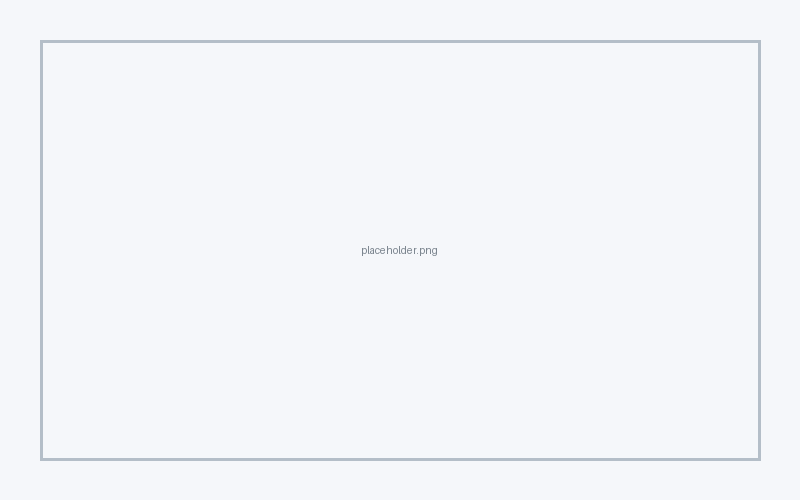
\includegraphics[width=0.75\textwidth]{placeholder.png}
    \caption{PNG 位图引用示例（如实验照片、截图等）}
    \label{fig:demo-png}
\end{figure}

Block Design 导出的 PDF 矢量图缩放无失真，推荐用于原理框图：

\begin{figure}[htbp]
    \centering
    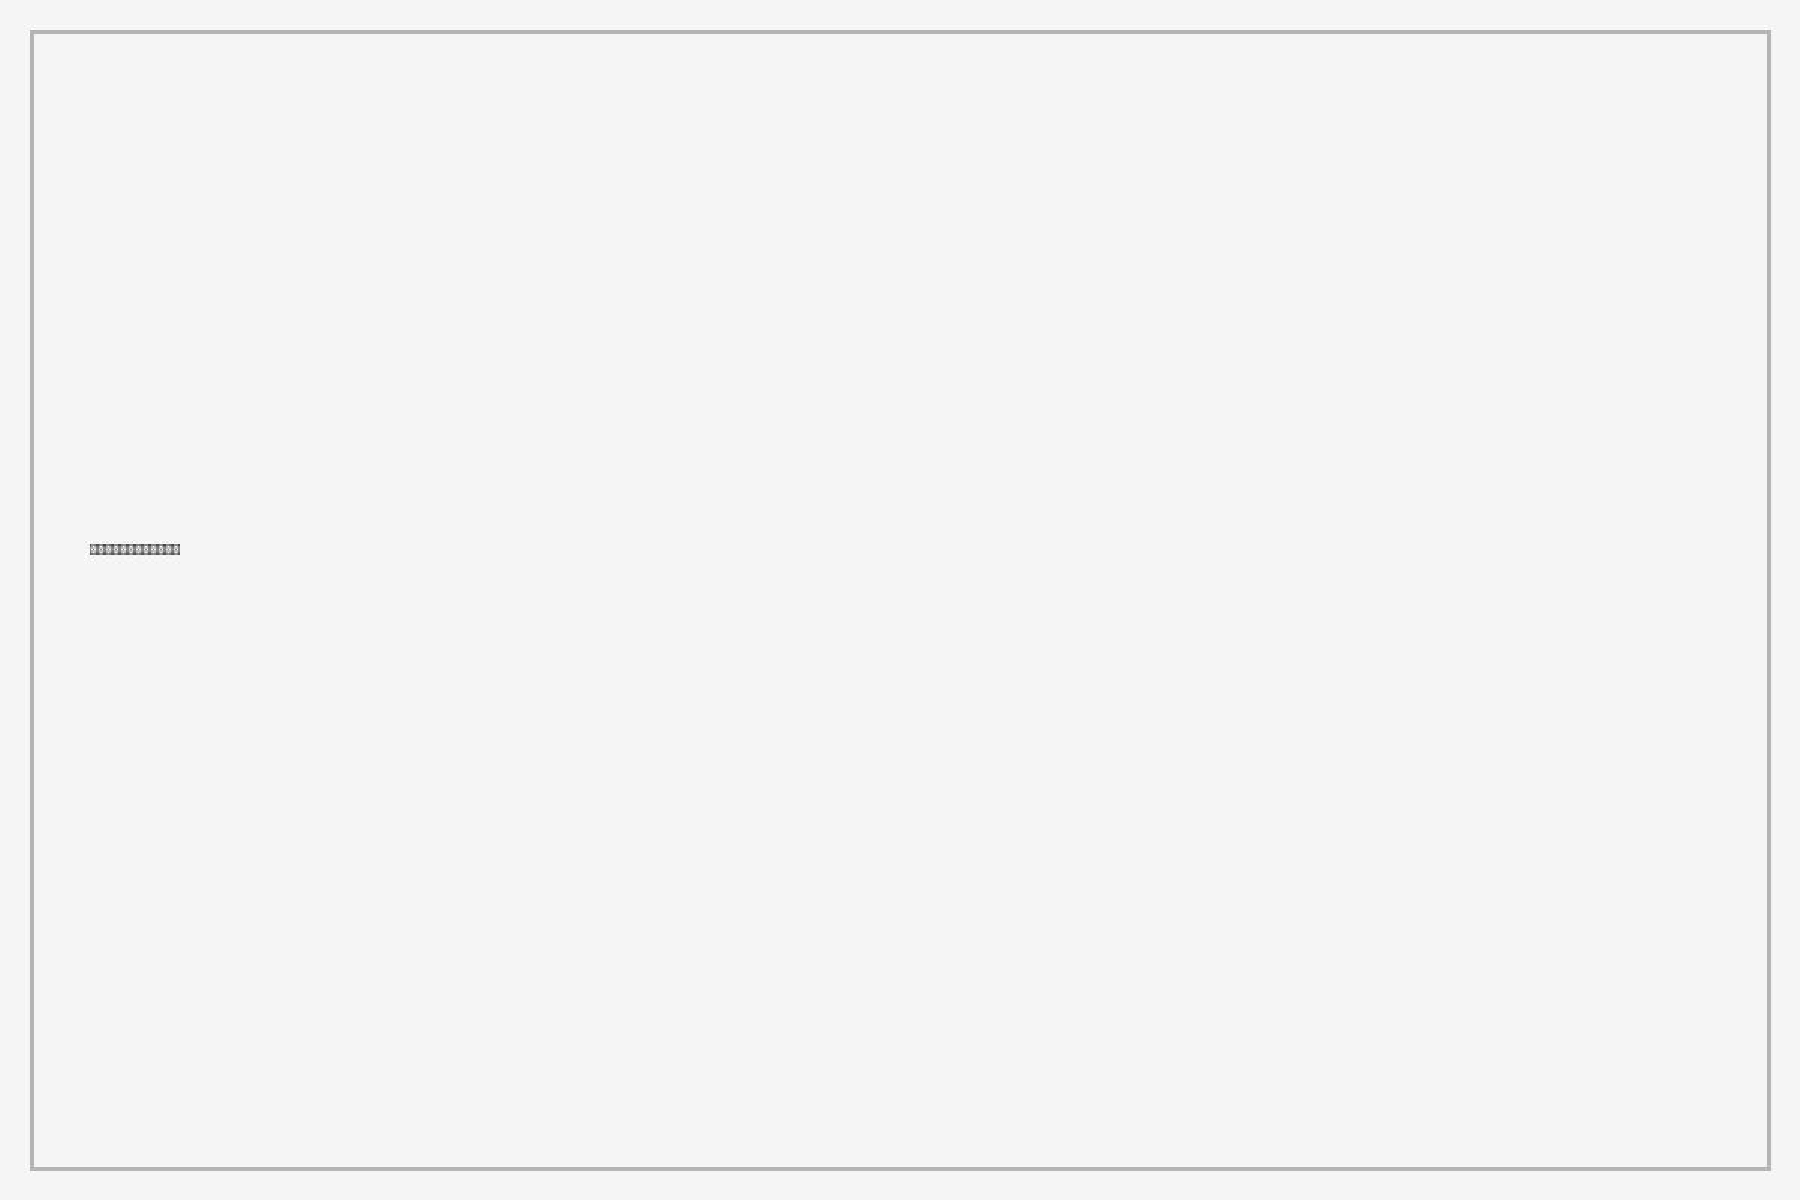
\includegraphics[width=0.9\textwidth]{placeholder.pdf}
    \caption{PDF 矢量图引用示例（如 Vivado Block Design 导出图）}
    \label{fig:demo-pdf}
\end{figure}

% ============================================================
%  4. 代码示例
% ============================================================
\subsection{代码示例}

代码块使用 VS Code Light+ 配色高亮，支持多种语言。代码颜色仅为语法区分，打印时浅色仍可辨认。

\blocktitle{（1）C 语言 — 嵌入式 GPIO 控制}
\begin{lstlisting}[
    style=vscode-c,
    caption={GPIO 输入输出示例程序},
    label={lst:c-gpio},
]
#include "xgpio.h"
#include "xil_io.h"
#include "xparameters.h"
#include <stdint.h>

static uint8_t seg_table[16] = {
    0x3F, 0x06, 0x5B, 0x4F, 0x66, 0x6D, 0x7D, 0x07,
    0x7F, 0x6F, 0x77, 0x7C, 0x39, 0x5E, 0x79, 0x71
};

int main(void)
{
    uint8_t sw_val = Xil_In8(XPAR_AXI_GPIO_0_BASEADDR);
    uint8_t digit  = sw_val & 0x0F;

    /* 将拨码低 4 位映射到七段码并输出 */
    Xil_Out8(XPAR_AXI_GPIO_1_BASEADDR, seg_table[digit]);

    while (1);  // 嵌入式主循环
    return 0;
}
\end{lstlisting}

\blocktitle{（2）Verilog — 数码管动态扫描（FPGA 必备）}
\begin{lstlisting}[
    style=vscode-verilog,
    caption={数码管动态扫描模块},
    label={lst:verilog-seg},
]
module seg_scan (
    input  wire        clk,        // 100 MHz 系统时钟
    input  wire        rst_n,      // 异步复位（低有效）
    input  wire [15:0] data,       // 4 位数码管数据
    output reg  [3:0]  seg_sel,    // 位选信号
    output reg  [7:0]  seg_code    // 段码输出
);

    reg [15:0] cnt;                // 分频计数器
    reg [1:0]  scan_idx;           // 扫描索引

    // 分频产生约 1 kHz 扫描时钟
    always @(posedge clk or negedge rst_n) begin
        if (!rst_n)
            cnt <= 16'd0;
        else if (cnt == 16'd49_999)
            cnt <= 16'd0;
        else
            cnt <= cnt + 1'b1;
    end

    wire scan_clk = (cnt == 16'd49_999);

    // 扫描状态机
    always @(posedge clk or negedge rst_n) begin
        if (!rst_n)
            scan_idx <= 2'd0;
        else if (scan_clk)
            scan_idx <= scan_idx + 1'b1;
    end

    // 位选译码
    always @(*) begin
        case (scan_idx)
            2'd0: seg_sel = 4'b1110;
            2'd1: seg_sel = 4'b1101;
            2'd2: seg_sel = 4'b1011;
            2'd3: seg_sel = 4'b0111;
            default: seg_sel = 4'b1111;
        endcase
    end

    // 段码输出（共阳极，低有效）
    always @(*) begin
        case (data[scan_idx*4 +: 4])
            4'h0: seg_code = 8'h3F;
            4'h1: seg_code = 8'h06;
            4'h2: seg_code = 8'h5B;
            4'h3: seg_code = 8'h4F;
            4'h4: seg_code = 8'h66;
            4'h5: seg_code = 8'h6D;
            4'h6: seg_code = 8'h7D;
            4'h7: seg_code = 8'h07;
            4'h8: seg_code = 8'h7F;
            4'h9: seg_code = 8'h6F;
            default: seg_code = 8'h00;
        endcase
    end

endmodule
\end{lstlisting}

\blocktitle{（3）Python — 数据处理脚本}
\begin{lstlisting}[
    style=vscode-python,
    caption={十六进制日志解析脚本},
    label={lst:py-parse},
]
from pathlib import Path
from typing import List


def parse_hex_line(line: str) -> int:
    """将一行十六进制字符串转为整数。"""
    return int(line.strip(), 16)


def load_values(path: Path) -> List[int]:
    """从文件读取并解析所有十六进制行。"""
    with path.open(encoding="utf-8") as f:
        return [parse_hex_line(ln) for ln in f if ln.strip()]


if __name__ == "__main__":
    data = load_values(Path("uart_log.txt"))
    print(f"共读取 {len(data)} 条记录，首项 = 0x{data[0]:02X}")
\end{lstlisting}

\blocktitle{（4）引用外部源文件}

推荐将源代码放在 \texttt{codes/} 目录，使用便捷命令引用（见 \coderef{lst:c-external}、\coderef{lst:py-external}）：

\includeC[caption={外部 C 源文件引用示例}, label={lst:c-external}]{codes/example.c}

\includePython[caption={外部 Python 源文件引用示例}, label={lst:py-external}]{codes/example.py}

% ============================================================
%  5. 交叉引用速查
% ============================================================
\subsection{交叉引用}

常用交叉引用命令汇总如下（编号均按章独立，随章节自动更新）：

\begin{itemize}
    \item \verb|\figref{fig:demo-png}| → \figref{fig:demo-png}
    \item \verb|\tabref{tab:module-resource}| → \tabref{tab:module-resource}
    \item \verb|\coderef{lst:c-gpio}| → \coderef{lst:c-gpio}
    \item \verb|\secref{sec:demo-text}| → \secref{sec:demo-text}
\end{itemize}

% ============================================================
%  附录示例
% ============================================================
\appendix

\section{附录示例：完整源代码}
\label{sec:appendix-source}

附录中的 section 编号自动变为「附录 A」「附录 B」…，写法与正文相同。

\includeC[caption={附录 A — GPIO 控制程序}, label={lst:appendix-c}]{codes/example.c}

\section{附录示例：Python 脚本}

\includePython[caption={附录 B — 数据处理脚本}, label={lst:appendix-py}]{codes/example.py}

% ============================================================ end 不要删除
\end{document}
